% asset_id: FAS1ComplexNumbersLociRegionsTikZ-003
\documentclass[tikz,border=8pt]{standalone}
\usepackage{amsmath}
\usepackage{xcolor}
\definecolor{Canvas}{HTML}{FAF9F6}
\definecolor{Ivory}{HTML}{FFFFF0}
\definecolor{SoftLine}{HTML}{E5E5EA}
\definecolor{TextInk}{HTML}{2C2C2E}
\definecolor{Gold}{HTML}{C5A059}
\definecolor{BrightGold}{HTML}{D4AF37}
\begin{document}
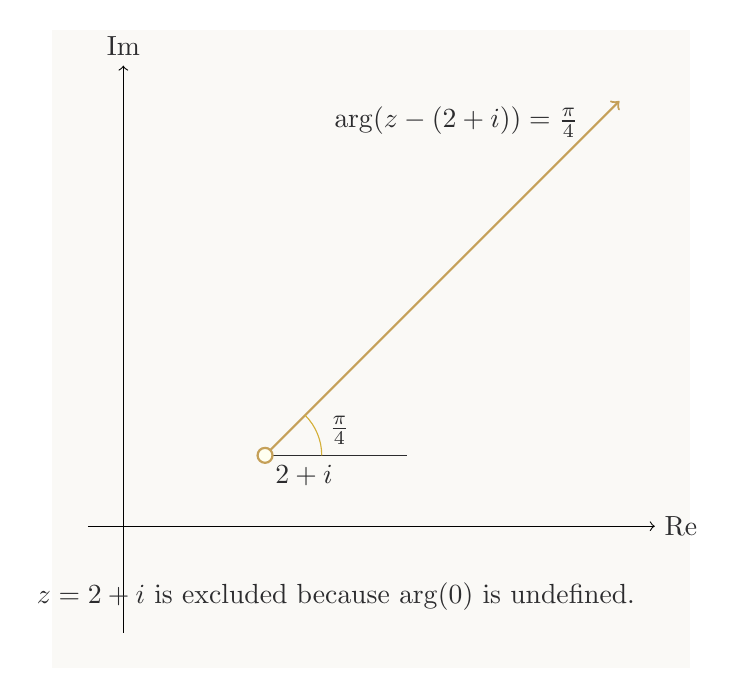
\begin{tikzpicture}[scale=0.9,every node/.style={text=TextInk}]
\fill[Canvas] (-1,-2) rectangle (8,7);
\draw[->] (-.5,0)--(7.5,0) node[right] {$\operatorname{Re}$};
\draw[->] (0,-1.5)--(0,6.5) node[above] {$\operatorname{Im}$};
\draw[Gold,thick,->] (2,1)--(7,6);
\draw[TextInk] (2,1)--(4,1);
\draw[BrightGold] (2.8,1) arc[start angle=0,end angle=45,radius=.8];
\node at (3.05,1.35) {$\frac{\pi}{4}$};
\draw[Gold,thick,fill=Ivory] (2,1) circle (3pt) node[below right] {$2+i$};
\node at (4.7,5.7) {$\arg(z-(2+i))=\frac{\pi}{4}$};
\node at (3,-1) {$z=2+i$ is excluded because $\arg(0)$ is undefined.};
\end{tikzpicture}
\end{document}
